\documentclass[11pt]{article}
\usepackage[a4paper,margin=1.1in]{geometry}
\usepackage[T1]{fontenc}
\usepackage[utf8]{inputenc}
\usepackage{lmodern}
\usepackage{microtype}
\usepackage{xcolor}
\usepackage{amsmath,amssymb,amsthm,booktabs}
\newtheorem{proposition}{Proposition}
\newtheorem{lemma}{Lemma}
\theoremstyle{definition}\newtheorem{observation}{Observation}
\theoremstyle{remark}\newtheorem{remark}{Remark}
\usepackage{graphicx}
\renewcommand{\topfraction}{0.9}\renewcommand{\floatpagefraction}{0.85}
\usepackage{tikz}
\usetikzlibrary{arrows.meta,positioning,calc,decorations.pathreplacing}
\usepackage[backend=biber,style=authoryear,maxcitenames=2,maxbibnames=6,giveninits=true,uniquename=false,uniquelist=false,doi=true,url=false,isbn=false]{biblatex}
\addbibresource{refs.bib}
\usepackage{hyperref}\hypersetup{colorlinks=true,linkcolor=black,citecolor=blue!50!black,urlcolor=blue!50!black}
\newcommand{\NUM}[1]{\textcolor{red!70!black}{\textbf{[NUM: #1]}}}
\newcommand{\EX}[1]{\textcolor{orange!80!black}{\textbf{[EX: #1]}}}
\title{How-possibly and how-actually:\\ what a resting-state manifold explains}
\author{P.~Mahon \\[2pt] \small Skeleton draft v3 (v2 sentences, reordered). \\ \small Every sentence is a draft for rewrite; conditional on the numerical gates.}
\date{17 November 2026}
\begin{document}
\maketitle

\section*{Opening}
\textcite{fousek2024} offer a mechanistic account of the brain's resting state. A network of bistable regions is coupled through a measured connectome and driven by noise. It settles onto a low-dimensional manifold, and the structured flow on that manifold produces the dynamic functional connectivity, the co-activation events and the cascades seen in resting fMRI and EEG. I will not dispute the model's internal analysis, which I think is sound. I will ask what kind of explanation the paper gives, and whether its evidence supports that kind. I will argue three things. The paper supplies a \emph{how-possibly} explanation of its phenomena, in \textcite{craver2006}'s sense: a model that shows how a mechanism could produce them. It presents this as a \emph{how-actually} explanation, one that shows how the mechanism does. And the strongest reply available to the authors relocates the problem rather than removing it. Stated as what it is, the paper is the first half of a well-formed explanatory project. The second half is testable and untested. A how-possibly model is a precondition of a how-actually one, not a failed version of it. A mechanism whose output is nowhere near the data is not a candidate at all. The question is what, beyond nearness, is needed. My answer in one line, in the terms of backward error analysis as \textcite{corless2016} and \textcite{fillion2014} present it: the paper establishes a backward error, that the data are the exact output of a nearby model, and reports it as a forward error, a bound on which models the data admit.

I will refer to the resting-state features the paper sets out to explain as `the phenomena', in the sense of \textcite{bogen1988}. I will call the network model `the mechanism' and the low-dimensional object it produces `the manifold'. First I will set out the paper's position, in its own words where I can, together with the best reply I can construct on the authors' behalf. Following this I will say where I agree with it, and what in it changed this critique. Then I will set out the objection. I will end with the two positions that I take to remain consistent.

\section{The position}
The brain at rest is modelled as a network of regions. Each region is a neural mass derived from a population of spiking neurons \parencite{montbrio2015}. Each is set in a regime with two stable states: a low-firing `down' state and a high-firing `up' state. The regions are coupled through a connectome measured by tractography, with conduction delays, and driven by noise. For weak coupling the regions switch independently and rarely. For strong coupling the network locks into the up state. In between, the heterogeneity of the connectome gives each region a different input, hence a different depth of its two wells, hence a different propensity to switch when its neighbours do. In that intermediate regime switches chain into cascades. Cascades produce bursts of co-activation in the slow BOLD signal, and the bursts recur. That recurrence is what dynamic functional connectivity records. The activity concentrates on a low-dimensional subset of the state space, the manifold. It is organised by the fixed points the connectome leaves stable and by their relative stability. The authors locate the regime by two statistics of the simulated BOLD: the variability of windowed functional connectivity across time, which they call fluidity, and the variance carried by two principal components. Both peak where the model's windowed-connectivity statistics are closest to an empirical session. The coincidence holds across a hundred subjects' connectomes. The regime also reproduces the event structure found in simultaneous EEG and fMRI.

The paper is explicit about what it wants. Earlier models, it says, ``leave a gap in the description of a mechanism''. To explain ``is not merely to redescribe one regularity \ldots\ as a series of several''. It is to reveal ``the productive relation between causal activities linked to their constituent entities'' \parencite[Introduction]{fousek2024}. This is mechanistic explanation in the sense of \textcite{mdc2000} and \textcite{craver2007}: entities (regions, tracts, bistable populations) and activities (noise-driven switching between up and down states), organized so as to produce the phenomenon. The standard carries its own tests. First, \textcite{craver2006} distinguishes a how-possibly model from a how-actually one. The first shows that a mechanism could produce the phenomenon; the second shows that it does. Only the second explains. The first is required for it, since the space of candidate mechanisms has to be charted before one can be singled out. \textcite{baetu2015} adds that interventions alone do not settle which of the two a model is; the completeness of the parts list matters. Second, the components of a how-actually model must be \emph{constitutively relevant}. Craver cashes this out as mutual manipulability: intervening on a part changes the whole, and intervening on the whole changes the part \parencite{craver2007}. The paper disclaims curve-fitting: ``our goal here is not to generate in silico observables that are as close as possible to the empirical one''. It does not disclaim realism. It asserts a mechanism of the brain.

On behalf of the authors one could put the position's defence as follows. I think it is the strongest reply available. The phenomena were never the warrant for the mechanism; they are the explanandum. The warrant comes from the independent evidence for the components, in the manner of \textcite{glymour1980}'s bootstrapping. In the numerical idiom it is a \emph{structured} backward error \parencite{highamhigham1992}: the measured components are pinned and only the unmeasured ones may vary. The connectome is measured, not fitted. The node model is derived exactly from spiking neurons. Bistable regional activity is reported in data \parencite[refs 39--41 therein]{fousek2024}. The feature match establishes sufficiency, which is all it was asked to establish. Constitutive relevance is shown by manipulation. Sweep the coupling and the phenomena come and go; replace the connectome with an all-to-all network and they vanish. Moreover, a stationary Gaussian process that matches the phenomena is a \emph{phenomenal} model in Craver's own sense, his Ptolemaic case. It is descriptively adequate and explanatorily empty, because it posits no components \parencite{craver2006}. It cannot compete with a mechanism, so it cannot underdetermine one. The relevant contrast class is mechanisms with independently warranted parts. That class is far smaller than ``all generators''. And the manifold is not a fitted object. It is a representational bridge between the parts and the phenomena, and it earns its keep by yielding predictions outside the phenomena used for selection. The up-state frequency should rise with a region's in-strength. The time spent in cascades should fall along the cortical hierarchy. Each subject's connectome should fix that subject's working point. On Lakatos's criterion, novel prediction is the mark of a progressive programme \parencite{lakatos1970}.

\section{Agreement}
I accept the standard. Holding the paper to a standard it chose is the fairest test available. I do not dispute the fixed-point and escape-time analysis, which stands on its own. At the stated parameters a node has a deep down state and a shallow up state at zero input. Input of order one-half equalises the two dwell times at a few seconds. Input above about 1.9 removes the down state altogether (Appendix~B). A region's dwell times are therefore set by its input, and its input by its in-strength times how many of its neighbours are up. That is what a cascade is, and it is a genuine mechanism. The frequency law is a falsifiable prediction. I also accept the cross-modal result inherited from the earlier paper: cascades in EEG precede co-activation events in BOLD. It survived the authors' own surrogate test \parencite{rabuffo2021}. No analysis of BOLD alone can address it, and it is the right shape for the rest of the programme.

\section{What changed this critique}
I think the reply of \S1 is right about two things. A phenomenal surrogate cannot refute a mechanism. And the dart board must be thrown over mechanisms, not over descriptions. My first version of this critique treated a stationary Gaussian process as a rival to the mechanism. It is not. The contrast class is the class of mechanisms.

The second thing is numerical. I reimplemented the model on a public 76-region connectome and built a stationary surrogate of the model's own BOLD. The surrogate attains the two-component share exactly, as it must, since that statistic is a function of the covariance alone. But at the working point the surrogate's fluidity index falls well short of the model's, between a quarter and a half of it in the two mixed-state records, and the tail of its co-activation amplitudes is about a third of the model's (Figure~\ref{fig:g1}; Appendix~C). Where the switching is real, the fluidity index sees it. The statistic is finer than I had allowed, and the objection is narrower accordingly.

\begin{figure}[htbp]\centering
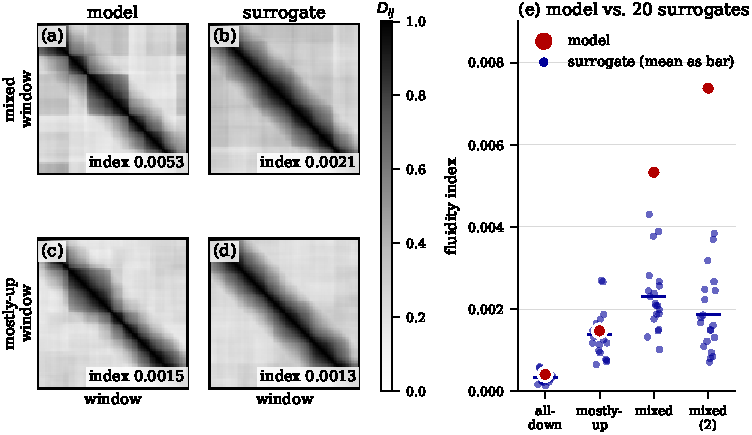
\includegraphics[width=\textwidth]{fig_g1.pdf}
\caption{Windowed-connectivity correlation matrices and the fluidity index, model against stationary surrogate. Panels (a)--(d): the matrix $D_{ij}$ of correlations between the connectivity vectors of windows $i$ and $j$ (window 60\,s, step 2\,s), for one 300\,s record of the reimplemented model at $G=0.9$, $\sigma=0.18$ in the mixed state (a) and in the mostly-up state (c), and for one cross-spectrum-preserving phase-randomised surrogate of each record (b, d), namely the one of twenty whose index lies nearest the ensemble median. Grey scale: $D_{ij}$ from 0 to 1. The number in each panel is that record's fluidity index, the variance of $D_{ij}$ over pairs at least a window apart. Panel (e): the fluidity index of the model record (large mark) and of its twenty surrogates (small marks; the bar is their mean) for the all-down, mostly-up and mixed states, and for a second mixed-state record started from a different initial condition. Each surrogate has the covariance and the spectra of its record.}
\label{fig:g1}
\end{figure}

\section{The objection}
Definitions first. By `data' I mean the recorded BOLD and EEG time series. By `phenomena' I mean, following \textcite{bogen1988}, the stable patterns extracted from data by a procedure. Here they are the fluidity of sliding-window functional connectivity, the share of variance carried by two principal components, and the statistics of high-amplitude co-activation events. A phenomenon is only as fine as the statistic that defines it.

\EX{a homely case of data versus phenomenon: the readings of a bathroom scale versus ``I have lost weight this month''; the second is what a diet explains, and it is only as fine as the averaging that produced it.}

Three facts about these particular phenomena will matter. The variance share of two components is a function of the sample covariance alone. The histogram statistic used to match model to data depends only on the multiset of correlation values, not on their order in time. The fluidity index is nearly order-free as well. It is positive for any stationary signal, because windowed correlations are noisy estimates with correlated errors. (The invariance statements are in \S4 and Appendix~A.) None of the three can tell a static covariance with autocorrelation from switching dynamics by its form alone. What the reimplementation shows is that the fluidity index can tell them apart by its \emph{magnitude} at the working point.

Here is the objection in its plainest form. The phenomena are coarse functionals of the data, and many generative hypotheses entail the same values of those functionals. A stationary Gaussian process with the right covariance and spectrum reproduces windowed dFC statistics \parencite{hindriks2016,liegeois2017,laumann2017} and co-activation events \parencite{novelli2022}. Simple linear models on the same connectome predict functional connectivity as well as nonlinear network models \parencite{messe2014,messe2015}. In mechanistic models generally, most parameter directions barely move the predictions \parencite{gutenkunst2007,machta2013,transtrum2015}, so disparate parameter sets yield the same activity \parencite{prinz2004}. The dart board in coupling and noise is small; the dart board that matters is over mechanisms, and that is what the surrogate and rewiring gates address (Appendix~C).

I want to be precise about which underdetermination this is. It is not the Duhem--Quine kind, where any hypothesis can be saved by adjusting auxiliaries. It is \emph{contrastive}, in the sense \textcite{laudan1991} separate from holism: the evidence fails to discriminate the proposed mechanism from a wide class of alternatives that entail the same phenomena. The inference from ``the model produces the phenomena'' to ``the model's mechanism is the brain's'' is then an inference to \emph{an} explanation, not to the best \parencite{lipton2004}. In Craver's terms, a how-possibly model has been offered as how-actually. I will refer to this as `the dart-board objection'. Throw a dart at the space of models and you hit one that reproduces the phenomena.

\EX{the dart board itself, or a lock that many keys open.}

The same point can be put in the language of backward error analysis, which I find clearer. \textcite{corless2016} and \textcite{fillion2014} present that analysis as an epistemology of modelling, not only a tool for algorithms. Three objects. First, the model. Write $\Psi$ for the map that takes a parameter setting $\theta$ (coupling, noise, connectome, node regime) to the law of the BOLD record the model generates at that setting. In practice: run the model and record the BOLD. Second, the statistic. Write $\varphi$ for the map that takes a BOLD record to the number or numbers that define a phenomenon. In practice: compute the fluidity index, or the two-component share. Third, the coordinates that matter. Write $\pi(\theta)$ for the part of $\theta$ that says which mechanism it is: the regime, the coupling structure, the noise law, as against the part that only tunes it. In symbols,
\begin{equation}
y \mapsto \varphi(y)\in\mathbb{R}^{k}, \qquad \theta \mapsto \varphi(\Psi(\theta)), \qquad \theta \mapsto \pi(\theta),
\label{eq:objects}
\end{equation}
and the composite $\varphi\circ\Psi$ is the object of study.

The backward-error question, in the form \textcite{corless2016} give it after \textcite{wilkinson1963}, is whether the computed answer is the exact answer to a nearby problem. Here it is whether the data are the exact output of a nearby model, with distance measured by the statistic. Corless and Fillion then say what is left once that question is answered. The task becomes ``whether or not the modified problem is a good model for the phenomenon being studied''. The first part is computation. The second is the modeller's judgement, and backward error analysis does not make it for you \parencite{fillion2014}. Their concluding gloss is the most charitable reading of the paper available: backward error analysis ``interprets the computed solution $z$ as the exact solution to just as good a model''. Whether the nearby model is just as good is the whole question. They add two cautions. A residual can be zero and the solution still wrong, when there are several solutions and nothing picks the right one. And a small residual is not enough without the sensitivity of the model to perturbation, ``even if $\Delta\equiv 0$''. Define
\begin{equation}
\beta(y)\;=\;\inf_{\theta}\,\bigl\|\varphi(\Psi(\theta))-\varphi(y)\bigr\|,
\qquad
A_{\varepsilon}\;=\;\bigl\{\theta \;\big|\; \|\varphi(\Psi(\theta))-\varphi(y)\|\le\varepsilon\bigr\}.
\label{eq:beta}
\end{equation}
Read: $\beta$ is how close the nearest model comes to the data on the phenomenon, and $A_\varepsilon$ is the set of all models that come within $\varepsilon$. The paper establishes that $\beta$ is small at its working point. In econometric language $A_0$ is the identified set \parencite{koopmans1950,manski2003}: what the phenomenon alone can tell you about the parameters, with unlimited data.

What how-actually requires is a bound on the \emph{forward} error: the size of $A_\varepsilon$ in the coordinates that distinguish mechanisms. This is Corless and Fillion's second caution, the sensitivity that has to be assessed even when the residual is zero. Forward error is backward error times a condition number \parencite{higham2002,corless2016}:
\begin{equation}
\operatorname{diam}\,\pi(A_{\varepsilon})\;\le\;\kappa\,\varepsilon,
\qquad
\kappa \;=\; 1\big/\sigma_{\min}\!\bigl(D(\varphi\circ\Psi)\big|_{\pi}\bigr),
\label{eq:forward}
\end{equation}
where $\sigma_{\min}$ is the smallest singular value of the Jacobian of $\varphi\circ\Psi$ restricted to the mechanism directions. Read: two mechanisms can both fit within $\varepsilon$ and still be $\kappa\varepsilon$ apart. For models of this kind the singular values span many decades \parencite{gutenkunst2007,machta2013,transtrum2015}, so $\kappa$ is large along most directions. That is the sloppiness result, and it is why disparate parameter sets yield the same activity \parencite{prinz2004}. Corless and Fillion's first caution, several solutions and nothing to pick the right one, can be made exact. It is best stated in the vocabulary of identification theory \parencite{rothenberg1971}. Two parameter values are \emph{observationally equivalent} with respect to a statistic when they induce the same law of that statistic. A parameter direction is \emph{identified} only if no such equivalence runs along it.

Take the two-component share as the case. It is a function of the sample covariance alone, so it is unchanged by every transformation of the record that preserves the covariance: permuting the samples, or replacing the record by any process with the same covariance, a stationary Gaussian one included.

\begin{proposition}[non-identification along the kernel]
Let $\varphi$ be invariant under a group $K$ of transformations of the data. Let $v$ be a direction in parameter space along which the law moves within a $K$-orbit: $\Psi(\theta+tv)=g_t\,\Psi(\theta)$ with $g_t\in K$. Then every $\theta+tv$ is observationally equivalent to $\theta$ with respect to $\varphi$. The information matrix of the induced family is singular along $v$, so $v$ is not identified by $\varphi$, locally or globally. And the compatible set $A_\varepsilon$ contains the whole line $\theta+\mathbb{R}v$ for every $\varepsilon\ge 0$.
\end{proposition}
The argument is short. Invariance gives $\varphi\circ g_t=\varphi$. So the law of $\varphi$ under $\Psi(\theta+tv)=g_t\Psi(\theta)$ equals its law under $\Psi(\theta)$ for every $t$; that is observational equivalence. The map $t\mapsto\varphi(\Psi(\theta+tv))$ is then constant and its derivative is zero. The information matrix is the Gram matrix of these derivatives, so it has $v$ in its null space, and by Rothenberg's rank condition $v$ is not locally identified. Since the equivalence holds for all $t$, it is not globally identified either. Constancy along the line puts the line inside $A_\varepsilon$.

In the vocabulary above the same fact reads: $\sigma_{\min}$ in \eqref{eq:forward} is zero along $v$, the condition number is infinite, and no backward error, however small, bounds the forward error in that direction. Identification is relative to the parameter space. The proposition bites when $\Theta$ contains directions that move the law at fixed covariance. The paper's own grid in $(G,\sigma)$ may not. The class of mechanisms under discussion does: it includes the covariance-matched Gaussian process and the near-Hopf and excitable regimes on the same connectome.

The same invariance holds for the paper's selection statistics; the statements are in Appendix~A. The histogram statistic depends only on the multiset of window-pair correlations, so reordering the windows in time leaves it unchanged. The fluidity index depends on the multiset over window pairs at least a window apart, so nearly the same holds for it. In words, the proposition says that these statistics have a kernel: a set of changes to the data they cannot register. Along the kernel no amount of fit constrains the mechanism. It does not say that the statistics register nothing. In the reimplementation the fluidity index at the mixed working point is two to four times its value on the covariance-matched surrogate (Figure~\ref{fig:g1}). It responds to the switching through its \emph{magnitude}, not its form. The kernel is real; it is not everything.

The null is also computable, which the paper does not do. For a stationary process the fluidity index has a floor. The connectivity estimated in a window is the true connectivity plus an estimation error; two windows a window apart have independent errors; and the index is then an inner product of two noisy unit vectors. Its mean and variance under that null follow from the law of the error alone, and in the limit of weak true connectivity the floor is one over the effective number of independent connectivity entries (Appendix~A). The floor is the tolerance $\varepsilon$ that \S5 asks for; it exists, and it can be reported.

The distinction is not new under other names. It is the econometrician's distinction between an identified set and point identification \parencite{koopmans1950,manski2003}. The set of parameters compatible with the data is Manski's identified set, and the paper's phenomena identify the mechanism only partially. Manski himself has recently connected partial identification to underdetermination \parencite{manski2026}. It is also Hadamard's distinction between an inverse problem that has a solution and one whose solution is unique and stable \parencite{engl1996}. Craver's distinction belongs beside those two.

\begin{figure}[htbp]\centering
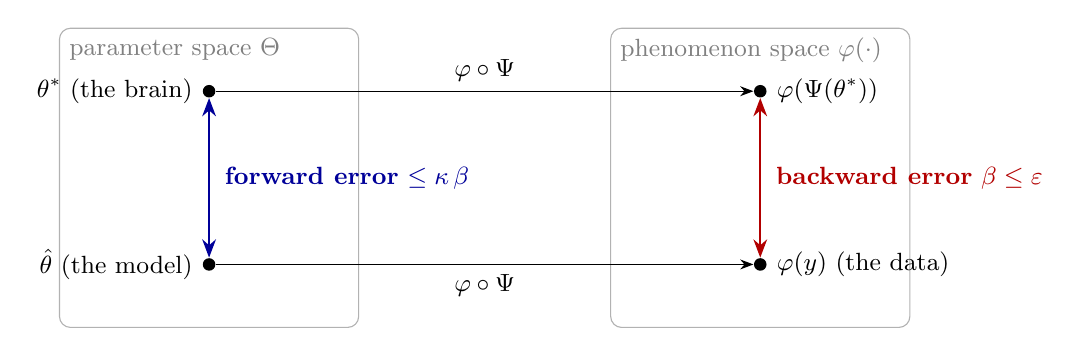
\begin{tikzpicture}[>=Stealth, node distance=1.2cm, font=\small]
  % spaces
  \draw[rounded corners, gray!60] (-0.4,-2.2) rectangle (3.4,1.6);
  \node[gray, anchor=north west] at (-0.4,1.6) {parameter space $\Theta$};
  \draw[rounded corners, gray!60] (6.6,-2.2) rectangle (10.4,1.6);
  \node[gray, anchor=north west] at (6.6,1.6) {phenomenon space $\varphi(\cdot)$};
  % points
  \node[circle,fill,inner sep=1.6pt,label=left:{$\theta^{*}$ (the brain)}] (ts) at (1.5,0.8) {};
  \node[circle,fill,inner sep=1.6pt,label=left:{$\hat\theta$ (the model)}] (th) at (1.5,-1.4) {};
  \node[circle,fill,inner sep=1.6pt,label=right:{$\varphi(\Psi(\theta^{*}))$}] (ps) at (8.5,0.8) {};
  \node[circle,fill,inner sep=1.6pt,label=right:{$\varphi(y)$ (the data)}] (py) at (8.5,-1.4) {};
  % maps
  \draw[->] (ts) -- node[above]{$\varphi\circ\Psi$} (ps);
  \draw[->] (th) -- node[below]{$\varphi\circ\Psi$} (py);
  % errors
  \draw[<->, thick, red!70!black] (ps) -- node[right, xshift=2pt]{\textbf{backward error} $\beta\le\varepsilon$} (py);
  \draw[<->, thick, blue!60!black] (ts) -- node[right, xshift=2pt]{\textbf{forward error} $\le\kappa\,\beta$} (th);
\end{tikzpicture}
\caption{Backward and forward error, in the layout of the commutative diagram of \textcite[\S2]{corless2016}, which follows \textcite[Fig.~1.1]{higham2002}, with the labels changed. Left box: parameter space $\Theta$, with the brain's parameters $\theta^{*}$ and the model's $\hat\theta$. Right box: the space of values of the statistic $\varphi$, with the output of each under the map $\varphi\circ\Psi$ (horizontal arrows) and the observed value $\varphi(y)$. The red arrow is the backward error $\beta$, the distance in the right-hand space between the data and the model's output; the blue arrow is the forward error, the distance in the left-hand space between the model's parameters and the brain's. The inequality on the blue arrow is Higham's bound, forward error $\le \kappa\,\beta$, with $\kappa$ the condition number of $\varphi\circ\Psi$.}
\label{fig:bf}
\end{figure}



Granting the phenomenal/mechanistic distinction of \S1 relocates the underdetermination without dissolving it, for three reasons.
\begin{enumerate}
\item The class of mechanisms with warranted parts that entail these phenomena is still large. Regions near a Hopf bifurcation, excitable regions, and metastable regimes on the same connectome all reproduce dynamic functional connectivity \parencite{hansen2015,deco2017,messe2015}. These are conceived alternatives, not Stanford's unconceived ones \parencite{stanford2006}, so the burden of discriminating among them is live now.
\item Bootstrapping requires that each component be warranted \emph{in the regime the mechanism invokes}. The connectome is. The bistable regime is a parameter choice the authors themselves describe as characteristic of sleep. Regional homogeneity is known to be false. The noise is unmeasured. The component with the least independent warrant is exactly the activity the mechanism needs: noise-driven switching between up and down states in the awake resting brain.
\item The novel predictions would settle the matter. But the frequency law is checked inside the model, and the hierarchy trend is reported without a test; the authors say its spatial match was not recovered. The per-subject result correlates two quantities that peak together by construction. One test the authors could run is in the reimplementation: permute the connectome's weights within each row, so that every region keeps its in-strength and the topology is scrambled. In five such connectomes, from three initial conditions each, the network fell to the all-down state every time, where the original connectome reaches the mostly-up and the mixed states. So in-strength alone does not fix the basins; that is a point for the authors. The rest of that test is in Appendix~C: matching the connectome's leading eigenvalue as well recovers part of the effect and not the basins.
\end{enumerate}

The explanation is therefore constitutive in form and how-possibly in evidential status.

\begin{figure}[htbp]\centering
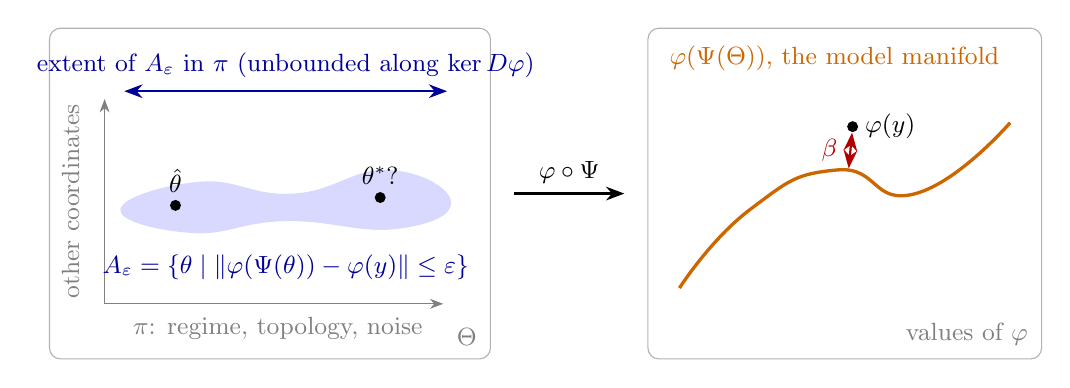
\begin{tikzpicture}[>=Stealth, font=\small]
  % ---- left box: parameter space
  \draw[rounded corners, gray!60] (0,0) rectangle (5.6,4.2);
  \node[gray, anchor=south east] at (5.55,0.05) {$\Theta$};
  \draw[->, gray] (0.7,0.7) -- (5.0,0.7); \node[gray, anchor=north] at (2.9,0.65) {$\pi$: regime, topology, noise};
  \draw[->, gray] (0.7,0.7) -- (0.7,3.3); \node[gray, rotate=90, anchor=south] at (0.5,2.0) {other coordinates};
  \fill[blue!15] plot[smooth cycle, tension=0.8] coordinates {(0.9,1.9) (1.9,2.25) (3.1,2.1) (4.3,2.4) (5.1,2.0) (4.4,1.65) (3.0,1.75) (1.8,1.6)};
  \node[blue!60!black, anchor=north] at (3.0,1.45) {$A_\varepsilon=\{\theta \mid \|\varphi(\Psi(\theta))-\varphi(y)\|\le\varepsilon\}$};
  \node[circle,fill,inner sep=1.4pt] at (1.6,1.95) {}; \node[above=1pt] at (1.6,1.95) {$\hat\theta$};
  \node[circle,fill,inner sep=1.4pt] at (4.2,2.05) {}; \node[above=1pt] at (4.2,2.05) {$\theta^{*}$?};
  \draw[<->, blue!60!black, thick] (0.95,3.4) -- (5.05,3.4);
  \node[blue!60!black, anchor=south] at (3.0,3.45) {extent of $A_\varepsilon$ in $\pi$ (unbounded along $\ker D\varphi$)};
  % ---- map
  \draw[->, thick] (5.9,2.1) -- node[above]{$\varphi\circ\Psi$} (7.3,2.1);
  % ---- right box: statistic space
  \draw[rounded corners, gray!60] (7.6,0) rectangle (12.6,4.2);
  \node[gray, anchor=south east] at (12.55,0.05) {values of $\varphi$};
  \draw[very thick, orange!80!black] plot[smooth, tension=0.9] coordinates {(8.0,0.9) (8.9,1.9) (10.0,2.4) (11.0,2.1) (12.2,3.0)};
  \node[orange!80!black, anchor=north west, align=left] at (7.75,4.1) {$\varphi(\Psi(\Theta))$, the model manifold};
  \node[circle,fill,inner sep=1.4pt] (d) at (10.2,2.95) {}; \node[right=1pt] at (d) {$\varphi(y)$};
  \draw[<->, red!70!black, thick] (d) -- node[left, xshift=-1pt]{$\beta$} (10.15,2.42);
\end{tikzpicture}
\caption{The compatible set and the model manifold. Left box: parameter space $\Theta$, drawn with the mechanism-distinguishing coordinates $\pi$ (regime, topology, noise) horizontal and the remaining coordinates vertical. The shaded region is the set $A_\varepsilon$ of parameters whose output lies within $\varepsilon$ of the data; $\hat\theta$ is one point of it, and $\theta^{*}$ is marked with a question mark because the data do not locate it within the region. The blue arrow spans the region's extent in $\pi$. Right box: the space of values of the statistic; the orange curve is the image $\varphi(\Psi(\Theta))$ of all of parameter space under the map (the model manifold, drawn as a curve because its width is small compared with its length, as in \textcite{transtrum2015}); the black point is the data $\varphi(y)$ and the red arrow is its distance $\beta$ to the manifold. The map $\varphi\circ\Psi$ sends the left box to the orange curve; the shaded region on the left is the preimage of the $\varepsilon$-neighbourhood of $\varphi(y)$ on the right.}
\label{fig:fibre}
\end{figure}

\section{Two positions that remain}
Two positions survive, and they are not the same paper.

The constructive-empiricist position \parencite{vanfraassen1980}: the model is empirically adequate with respect to the chosen observables, and the manifold is a device for thinking about the model. This is consistent, but it has a cost. Adequacy is relative to observables, and these observables cannot register the device's distinctive content, so adequacy is cheap, and ``the brain's resting state manifold'' becomes a manner of speaking. On this reading the paper's title claims more than its position allows.

The realist position, which the authors take: the manifold and the switching mechanism are in the brain. Then what is owed is the how-actually programme that the reply of \S1 itself describes. Intervening on the system would settle the matter: an intervention adds an equation the compatible set must satisfy, and it is the test Craver's criterion asks for. For this phenomenon it is not available, and no reasonable critique can demand it. That leaves four ways to shrink the set of models the data admit, in the terms of \S4. They are not the same move.
\begin{enumerate}
\item Refine the statistic until its kernel is small: a finer norm.
\item Pin more components by independent measurement in the regime invoked: a smaller parameter space.
\item Add equations the fibre must also satisfy: cross-modal constraints, and any further observable the mechanism is committed to.
\item Weight the fibre by a stated reference measure: a posterior, which does not shrink the set but says how much of it one believes.
\end{enumerate}
Concretely: warrant the activity independently, or restrict the scope to states where up/down bistability is established and test whether the cascade and connectivity signatures track it across sleep stages. Test the derived predictions outside the model: up-state frequency against in-strength in source-localized MEG, and per-subject working points out of sample. Select and validate on observables that can see the object, the dwell-time and transition structure along the axis of global activation. Discriminate among mechanistic rivals on those observables by model comparison or simulation-based inference, which the group already has \parencite{hashemi2024}.

The choice of statistic is itself a problem with a solution, and it is where Corless and Fillion's two cautions meet. Coarsen $\varphi$ and the backward error falls while the condition number rises. Refine it toward the likelihood and the condition number falls while the backward error rises, because the model is misspecified somewhere and nothing fits. The right statistic is the finest one at which the model remains adequate. At that statistic the compatible set is as small as this model class allows:
\begin{equation}
\varphi^{\dagger}\;=\;\arg\max_{\varphi}\ \sigma_{\min}\!\bigl(D(\varphi\circ\Psi)\big|_{\pi}\bigr)
\quad\text{subject to}\quad \beta_{\varphi}(y)\le\varepsilon .
\label{eq:design}
\end{equation}
Read: among the statistics the model can still match to within the data's own variability, take the one that separates mechanisms most. In inverse problems this rule has a name, Morozov's discrepancy principle: regularise no further than the noise level \parencite{engl1996}. In statistics it is the design of summary statistics \parencite{fearnhead2012}. In \textcite{mayo1996}'s terms it is severity: a test the mechanism would have failed had it been false. The reimplementation suggests one such statistic: the ratio of the co-activation amplitude tail to that of its own phase-randomised surrogate. In the model's mixed state that ratio is about three, and in its mostly-up state between one and two (Appendix~C). In the authors' empirical data, by their own earlier test, the surrogate preserved the tail \parencite[Extended Data Fig.~9-1]{rabuffo2021}.

\begin{figure}[htbp]\centering
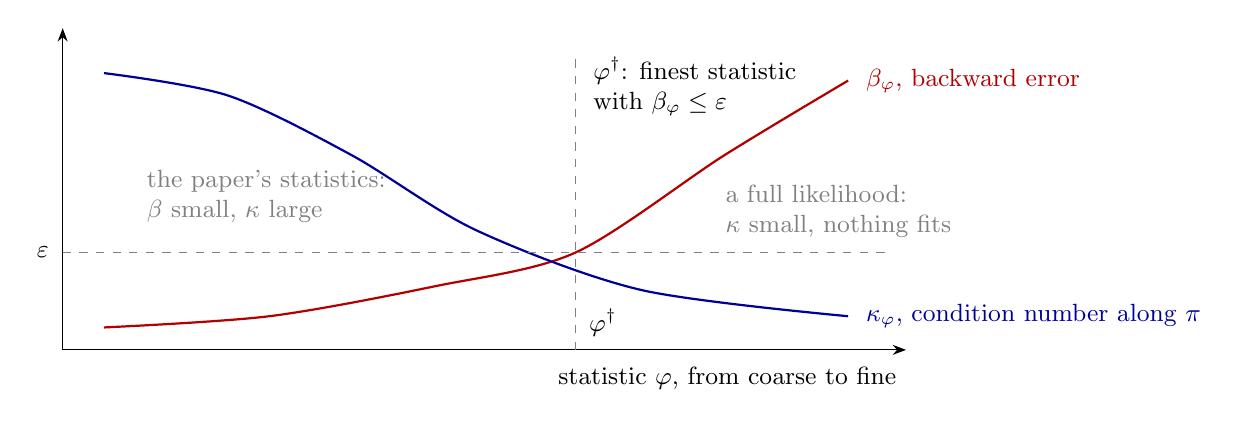
\begin{tikzpicture}[>=Stealth, font=\small, xscale=1.05, yscale=0.95]
  \draw[->] (0,0) -- (10.2,0); \node[anchor=north east] at (10.2,-0.1) {statistic $\varphi$, from coarse to fine};
  \draw[->] (0,0) -- (0,4.3);
  \draw[thick, red!70!black] plot[smooth] coordinates {(0.5,0.30) (2.5,0.45) (4.5,0.85) (6.2,1.30) (8.0,2.6) (9.5,3.6)};
  \node[red!70!black, anchor=west] at (9.6,3.6) {$\beta_\varphi$, backward error};
  \draw[thick, blue!60!black] plot[smooth] coordinates {(0.5,3.7) (2.0,3.4) (3.5,2.6) (5.0,1.6) (7.0,0.8) (9.5,0.45)};
  \node[blue!60!black, anchor=west] at (9.6,0.45) {$\kappa_\varphi$, condition number along $\pi$};
  \draw[dashed, gray] (0,1.3) -- (10.0,1.3); \node[anchor=east] at (-0.05,1.3) {$\varepsilon$};
  \draw[dashed, gray] (6.2,0) -- (6.2,3.9); \node[anchor=south west] at (6.25,0.05) {$\varphi^{\dagger}$};
  \node[gray, anchor=west, align=left] at (0.9,2.05) {the paper's statistics:\\ $\beta$ small, $\kappa$ large};
  \node[gray, anchor=west, align=left] at (7.9,1.85) {a full likelihood:\\ $\kappa$ small, nothing fits};
  \node[anchor=south west, align=left] at (6.3,3.0) {$\varphi^{\dagger}$: finest statistic\\ with $\beta_\varphi\le\varepsilon$};
\end{tikzpicture}
\caption{Backward error and condition number as the statistic is refined. Horizontal axis: the statistic $\varphi$, ordered from coarse (a few moments) to fine (a full likelihood); the ordering is schematic. Red curve: the backward error $\beta_\varphi$, the distance from the data to the model manifold measured in the seminorm of $\varphi$. Blue curve: the condition number $\kappa_\varphi$ of $\varphi\circ\Psi$ along the mechanism-distinguishing coordinates $\pi$. The horizontal dashed line is the tolerance $\varepsilon$ set by the sampling variability of $\varphi$; the vertical dashed line marks $\varphi^{\dagger}$, the finest statistic at which $\beta_\varphi\le\varepsilon$. The grey annotations place the paper's selection statistics near the coarse end and a full likelihood near the fine end.}
\label{fig:eq}
\end{figure}

Figure~\ref{fig:eq} draws the trade-off; Figure~\ref{fig:fibre} is what the left end of it looks like.

Stated that way, the paper is the how-possibly half of a well-formed project, and its real claim is the testable one it has not yet tested. I do not think that is a small thing to have done. I do think it is a different thing from what the title says.

\section{Limits of this critique}
What is said here does not touch the fixed-point and escape-time analysis, which stands on its own. It does not touch the cross-modal result, nor the authors' statement that they were not fitting. It touches the step from the model to the brain, and only that step. The numerical gates are model-internal, on a public 76-region connectome rather than the authors' subject, so they bear on the reimplementation and on the statistics, not on the paper's own runs. One request falls out of it that costs the authors nothing: the tolerance. The model's output is a law and the data are one sample path. So ``within tolerance'' needs the sampling variability of each statistic across sessions or subjects. Without that number the set of admitted models has no boundary, and neither this critique nor the paper's claim can be made quantitative.


\appendix
\section{Invariance statements and the stationary floor}
Throughout, $y\in\mathbb{R}^{T\times N}$ is a BOLD record, $C(y)$ its sample covariance, $F_i$ the vectorised upper triangle of the correlation matrix of window $i$ (length $W$ samples, step one sample, as in the paper's Eqs.~6--8), $M=N(N-1)/2$, and $D_{ij}=\operatorname{corr}(F_i,F_j)$ across the $M$ entries.

\paragraph{What each selection statistic depends on.}
\begin{center}\small
\begin{tabular}{p{4.0cm}p{4.0cm}p{6.0cm}}
\toprule
statistic & depends on $y$ only through & hence unchanged by \\
\midrule
two-component share $\varphi_V$ & the eigenvalues of $C(y)$ & permutations of the $T$ samples; any process with the same covariance, including a stationary Gaussian one \\
histogram statistic (KS distance on the centred $D_{ij}$, $i<j$) & the multiset $\{D_{ij}\}$ & every permutation of the windows in time; dwell times and the order of recurrences \\
fluidity index $s=\operatorname{Var}\{D_{ij}\mid i\le j-W\}$ & the multiset over admissible pairs & window reversal; every permutation preserving the admissible pair set (not arbitrary reorderings, which change which pairs are admissible) \\
\bottomrule
\end{tabular}
\end{center}
The invariances are in the sense of \textcite[ch.~6]{lehmann2005}. Their consequence for identification is the Proposition of \S4.

\paragraph{Structured backward error.} Partition $\theta=(\theta_{\mathrm{pinned}},\theta_{\mathrm{free}})$ into components fixed by independent measurement and the rest. The structured backward error is
\[
\beta^{\mathrm{s}}(y)\;=\;\inf_{\theta_{\mathrm{free}}}\bigl\|\varphi\bigl(\Psi(\theta_{\mathrm{pinned}},\theta_{\mathrm{free}})\bigr)-\varphi(y)\bigr\| ,
\]
the structured analogue of \eqref{eq:beta} \parencite{highamhigham1992}. Pinning shrinks $A_\varepsilon$ only in the pinned coordinates. The authors' reply in \S1 is the claim that $\beta^{\mathrm{s}}$ is small with the connectome pinned, which is true, and leaves the regime and the noise free, which is the point of \S4.

\paragraph{The stationary floor of the fluidity index.} Write the connectivity vector of window $w$ as $F_w=\rho+e_w$, with $\rho$ the true connectivity and $e_w$ the estimation error; centre across entries, so that $v=\rho-\bar\rho$ and $e_w$ has mean zero and covariance $S$. For windows at least a window apart take the errors independent. Then $D_{ij}=u_i^{\top}u_j$ with $u_w=(v+e_w)/\|v+e_w\|$, and the $u_w$ are independent and identically distributed.
\begin{lemma}[stationary floor]
Under those assumptions, with $\mu=\mathbb{E}[u]$ and $Q=\mathbb{E}[uu^{\top}]$,
\[
\mathbb{E}[D_{ij}]=\|\mu\|^{2},\qquad \operatorname{Var}[D_{ij}]=\operatorname{tr}(Q^{2})-\|\mu\|^{4},
\]
exactly. In the limit of weak true connectivity, $v\to 0$, $\operatorname{Var}[D_{ij}]\to\operatorname{tr}(S^{2})/(\operatorname{tr}S)^{2}=1/M_{\mathrm{eff}}(S)$, the inverse participation ratio of the error covariance. To first order in $e$,
\[
\mathbb{E}[D_{ij}]\approx\frac{v^{\top}v}{v^{\top}v+\operatorname{tr}S},\qquad
\operatorname{Var}[D_{ij}]\approx\frac{2\,v^{\top}Sv+\operatorname{tr}(S^{2})}{(v^{\top}v+\operatorname{tr}S)^{2}} .
\]
\end{lemma}
The exact identities follow from independence: $\mathbb{E}[u_i^{\top}u_j]=\mu^{\top}\mu$ and $\mathbb{E}[(u_i^{\top}u_j)^{2}]=\mathbb{E}[u_i^{\top}u_ju_j^{\top}u_i]=\operatorname{tr}(Q^{2})$. The limit $v\to0$ makes $u$ a unit vector in the direction of $e$, and the first-order forms come from expanding the norms. For a stationary Gaussian process the error covariance is the asymptotic covariance of sample correlations \parencite{steiger1980} divided by an effective sample size that corrects for autocorrelation \parencite{bartlett1935}; in the model's regimes the effective size is about 17 of the 83 samples in a window.

\paragraph{Check against the exact null.} The exact null is the surrogate ensemble: phase randomisation with the cross-spectrum preserved gives a stationary Gaussian process with the record's own covariance and spectra, and the fluidity index computed on it is the floor without approximation. For the model's own regimes the floor, computed by surrogate, is 0.0023 and 0.0019 in the two mixed-state records, 0.0014 in the mostly-up state and 0.0003 in the all-down state. The model's values are 0.0053 to 0.0074, 0.0012 to 0.0026, and 0.0003 to 0.0005. For the three collective states of the reimplementation at $G=0.9$, $\sigma=0.18$ (twenty surrogates per record, the ensembles of Figure~\ref{fig:g1}; $\pm$ one standard deviation across surrogates):
\begin{center}\footnotesize
\begin{tabular}{@{}lcccc@{}}
\toprule
state & surrogate floor & model & lemma (exact-moment) & lemma (first order) \\
\midrule
mixed (0.36 up) & $0.0023\pm0.0008$ & $0.0053$ & $0.0034$ & $0.0065$ \\
mixed, 2nd record & $0.0019\pm0.0009$ & $0.0074$ & --- & --- \\
mostly-up (0.73 up) & $0.0014\pm0.0006$ & $0.0012$--$0.0026$ & $0.0027$ & $0.0039$ \\
all-down & $0.0003\pm0.0001$ & $0.0003$--$0.0005$ & $0.0013$ & $0.0011$ \\
\bottomrule
\end{tabular}
\end{center}
The plug-in evaluations take $v$ and $S$ at the estimated full-record correlation matrix and overshoot the exact null by a factor of two to four, because that estimate carries its own sampling noise into $v$ and $S$; a debiased plug-in is the next step and is not done.

\section{The model as implemented}
Regions follow the Montbri\'o--Paz\'o--Roxin equations with the paper's parameters ($\eta=-5$, $J=15$, $\Delta=1$, $\tau_c=1$; one time unit $=1$\,ms by the authors' convention), coupled as $I_i=G\sum_j W_{ij}\,r_j(t-D_{ij})$ with delays from tract lengths at 2\,m/s, additive Gaussian noise of standard deviation $\sigma$ per $\sqrt{\text{ms}}$ on both variables, Heun drift with Euler--Maruyama noise at $\mathrm{d}t=0.05$, and Balloon--Windkessel haemodynamics driven by the firing rate and sampled at TR\,$=720$\,ms. The connectome is the 76-region connectivity distributed with The Virtual Brain, weights scaled to unit mean in-strength. Statistics are coded from the paper's Eqs.~6--8.

\paragraph{One node at the paper's parameters.} From $\dot r=0$, $v=-\Delta/(2\pi r)$; substituting into $\dot v=0$ gives one equation in $r$.
\begin{center}\small
\begin{tabular}{cccc}
\toprule
input $I$ & down state $(r,v)$ and eigenvalues & saddle $r$ & up state $(r,v)$ and eigenvalues \\
\midrule
0 & $(0.081,-1.96)$; $-2.45$, $-5.40$ & $0.47$ & $(1.03,-0.15)$; $-0.31\pm3.32i$ \\
1 & $(0.098,-1.62)$; $-1.64$, $-4.84$ & $0.32$ & $(1.18,-0.14)$; $-0.27\pm4.40i$ \\
2 & gone & gone & $(1.28,-0.12)$; $-0.25\pm5.16i$ \\
5 & & & $(1.52,-0.11)$; $-0.21\pm6.76i$ \\
\bottomrule
\end{tabular}
\end{center}
The down state and the saddle meet near $I\approx1.87$. Mean escape times at $\sigma=0.18$ (single node, 100 trajectories): down$\to$up 8.8\,s at $I=0$, 1.5\,s at $0.25$, 0.27\,s at $0.5$, 49\,ms at $0.75$; up$\to$down 40\,ms at $0$, 0.13\,s at $0.25$, 0.42\,s at $0.5$, 1.0\,s at $0.75$, 3.1\,s at $1.0$. The two dwell times are equal near $I\approx0.5$.

\section{Pre-registered gates and results}
Each gate was written down with the outcome that would defeat the critique before it was run. All runs: 76-region public connectome, $\sigma=0.18$ unless stated, five minutes of model time, statistics as in Appendix~B.

\paragraph{G1 in numbers.} In two replicates of the mixed state the index is 0.0053 and 0.0074 against surrogate values of $0.0023\pm0.0008$ and $0.0019\pm0.0009$, and the 99th percentile of event amplitude is 0.40 and 0.33 of the model's. Twenty surrogates per record; in both mixed-state records the model's index exceeds every surrogate's. In the mostly-up state the model's index ranks thirteenth of twenty-one against its own surrogates, and in the all-down state eighteenth. The ratio of the model's event-amplitude tail to its surrogate's is about three in the mixed state (the surrogate's tail is 0.33 to 0.40 of the model's) and 1.2 to 1.7 in the mostly-up state.

\paragraph{G2 in full.} The permutation also lowers the leading eigenvalue of the connectome by twelve percent, which at fixed coupling is an under-coupled network, so the question becomes whether topology matters beyond that one number. Raising the coupling on a rewired connectome until the product with its leading eigenvalue matches the original answers in part: on two such connectomes, from three initial conditions each, the network settled in a switching mixed state three times and fell to all-down three times, and it never reached the mostly-up state, where the original reaches an up-containing state from every comparable start. In-strength and the leading eigenvalue together do not reproduce the basins. Something finer in the connectome, the reciprocity being the obvious candidate, sets their size. Two connectomes are too few to measure that size; they are enough to show it is not two numbers.

\paragraph{G4.} In the reimplementation the fluid band is narrow in the coupling, about a tenth of the grid at the right noise level, and inside it the collective state a run reaches depends on its initial condition.
\begin{center}\small
\begin{tabular}{@{}p{1.6cm}p{4.3cm}p{3.5cm}p{3.9cm}@{}}
\toprule
gate & question & defeats the critique if & result \\
\midrule
G0 & does the reimplementation show the paper's fluid band? & (positive control) no band: stop & band at $G\approx0.9$--$1.0$: switching index and two-component share rise together; flanked by all-down ($G\le0.7$) and all-up ($G\ge1.1$) \\
basins & is the working point a point? & --- & three stationary collective states at $G=0.9$: all-down, mixed (0.36 up), mostly-up (0.73); reached from different initial conditions \\
G1 & does a stationary surrogate attain the selection statistics? & surrogate's switching index well below the model's seed spread & fires in the mixed state (0.0019--0.0023 vs 0.0053--0.0074; event tail at 0.33--0.40); attained in the mostly-up state (0.0013--0.0024 vs 0.0012--0.0026) \\
G2 & does topology beyond in-strength matter? & band shifts or disappears under within-row rewiring & fires: five rewirings, fifteen runs, all all-down; rewiring also lowers $\lambda_1(W)$ by 12\%; $\lambda_1$-matched test (two permutations, $G=1.03$, three starts each): mixed state 3 of 6, all-down 3 of 6, mostly-up 0 of 6; partial return \\
G3 & does a two-state model with the full model's own flip rates reproduce the states? & cannot reach the model's statistics & partial: reproduces all-down and mostly-up (and the mostly-up statistics at $G=1.0$); not the mixed state in 16 runs; basin boundary shifted \\
G4 & acceptance fraction under a reference measure & (measurement) & fluid band $\approx$ a tenth of the coupling grid at the right noise; within it the state depends on initial condition; zero of fifteen rewired runs \\
\bottomrule
\end{tabular}
\end{center}

\printbibliography
\end{document}
